\documentclass{beamer}

\usepackage{graphicx}
\graphicspath{ {./images/} }
\usepackage{thm-restate}
\usepackage{textcomp}
\setbeamertemplate{theorems}[numbered]

%\usetheme{Madrid}
%\usetheme{Warsaw}
\usetheme{Copenhagen}

%\setbeamertemplate{footline}[frame number]{}
\setbeamertemplate{navigation symbols}{\insertframenumber/\inserttotalframenumber}

\newtheorem*{rquestion}{Question}
\newtheorem{subquestion}{Sub-Question}

\newcommand{\textapprox}{\raisebox{0.5ex}{\texttildelow}}

\title[Logistical Optimisation for Offshore Windfarms]{Simulation and Optimisation of Offshore Renewable Energy Arrays for Minimal Life-Cycle Costs}

\author{Robin Kuipers}

\date{October 27, 2020}

\begin{document}

\begin{frame}
  \titlepage
\end{frame}


\begin{frame}{The project}
  \begin{itemize}
  	\item Improve scheduling logistics of operations on modern windfarms in the North Sea
  	\item Literature tends to split the life-cycle in three phases
  	\begin{itemize}
  		\item Installation (\textapprox  2-3 years)
  		\item Maintenance (\textapprox 15-25 years)
  		\item Decommission (\textapprox 2-3 years)
  	\end{itemize}
  	\item Large industrial vessels used for major operations; small improvements can lead to large savings
	\item Most research in literature chooses a phase to focus on; my work looks at how the phases interact
  \end{itemize}
\end{frame}


\begin{frame}{Research Questions}
\small
\begin{rquestion}
Can considering the entirety of the life-cycle of an Offshore Wind Farm, and how each of the phases interact, improve logistical decision making on these projects?
\end{rquestion}

\bigskip

\begin{subquestion}
Can considering how phases in the life-cycle of a windfarm overlap and share resources improve logistical decision making on these projects?
\end{subquestion}

\begin{subquestion}
Can considering the entire life-cycle of a windfarm provide useful data to base logistical decisions on in the later phases of these projects?
\end{subquestion}

\begin{subquestion}
Can considering the long-term effects of logistical decisions early on in the life-cycle of a windfarm improve these decisions? 
\end{subquestion}
\end{frame}


\begin{frame}{Progress - Models}
\begin{itemize}
\item Developed individual deterministic optimization models for each phase
\item Combined models in lifespan model
\item Experimented with ways to make models stochastic and robust
\end{itemize}

\bigskip

\begin{itemize}
\item Implemented each of the models in C++ using Xpress
\item Used basic test cases to improve models and test sanity of solutions
\item Experimented with variants of models to improve computational efficiency
\end{itemize}
\end{frame}


\begin{frame}{Progress - Other}
\begin{itemize}
\item Increased my own knowledge reading literature
\item Focused on reading about maintenance scheduling
\item Gained access to extensive weather data
\item Helped teach a course
\item Followed an online course
\item Made an actionable plan to work towards first publication
\end{itemize}
\end{frame}


\begin{frame}{Direct focus}
\only<1,4>{
\setcounter{subquestion}{0}
\begin{subquestion}
Can considering how phases in the life-cycle of a windfarm overlap and share resources improve logistical decision making on these projects?
\end{subquestion} 

\onslide<4>{
\begin{figure}[t]
 	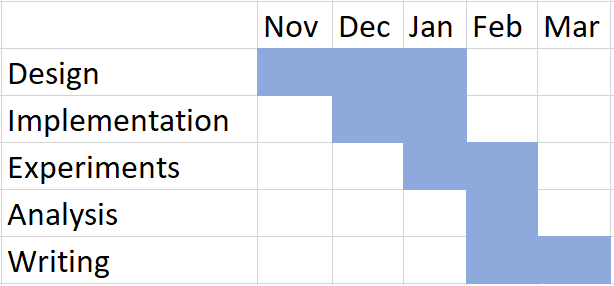
\includegraphics[width=0.75\textwidth]{gantt}
	\centering
\end{figure}}}

\only<2,3>{
\begin{figure}[t]
 	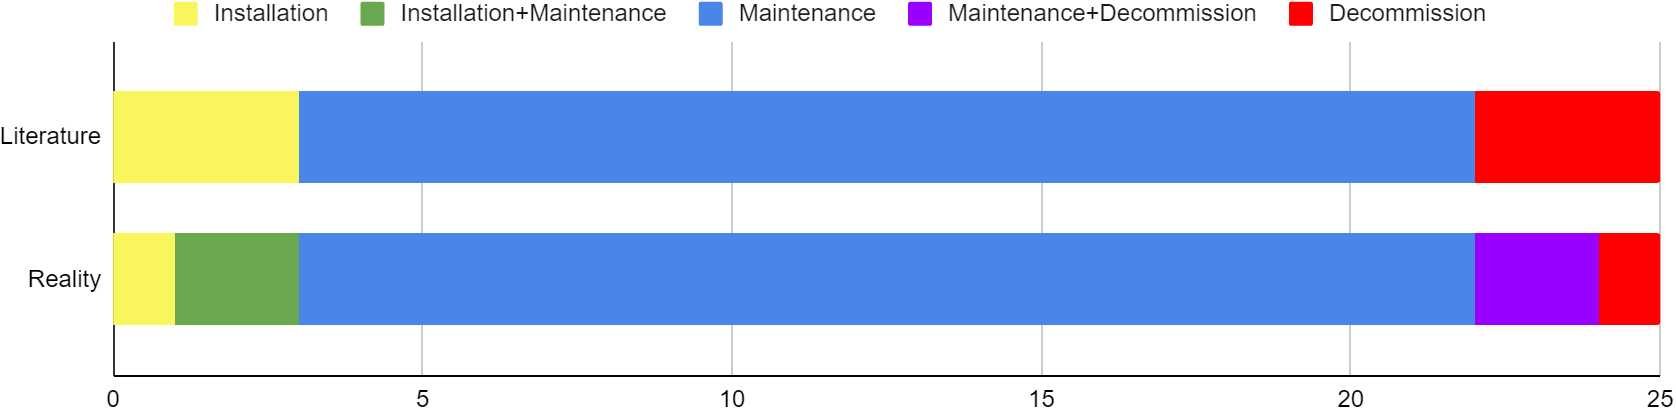
\includegraphics[width=1\textwidth]{overlapgraph}
	\centering
\end{figure}

\onslide<3>{
\begin{itemize}
\item Will investigate the time intervals at which phases overlap
\item During this time resources are shared
	\begin{itemize}
	\item Can lead to complications when ports or maximum amount of vessels are in use
	\item Can lead to optimizations when vessels can reduce idle time working on multiple phases
	\end{itemize}
\item The number of active turbines varies, potentially complicating maintenance
\item Overlap time \textit{might} have a disproportionate amount of failures
\end{itemize}}}
\end{frame}


\begin{frame}{Later work}
\begin{itemize}
\item Build simulation model for the life-cycle
\item Use this model to answer other sub-questions
\item Consider failure rate informed by individual (predicted) history of turbine
\end{itemize}

\bigskip

\begin{itemize}
\item Hopefully publish any significant results found
\item Finalize writing
\item Complete the project in the next 12 months
\end{itemize}

\bigskip

\pause
\begin{center}
 Thank you for listening!
\end{center}
\end{frame}

\end{document}


